\subsection{Tests Objekterkennung}
\label{sec_testObj}
\todo{bitte erst ab dritte Testreihe lesen}
Die Objekterkennung wurde auf drei Arten getestet. Für diese Arbeit ist eine verlässliche Erkennung auf Simulationsbildern wichtig. Aus diesem Grund beziehen sich die ersten Tests auf Simulationsbildern. Der dritte Test dient der Evaluation der genutzten Methode in Bezug auf Echtdaten.\\
Die erste Testreihe besteht aus Bildern, auf denen das Objekt gut zu sehen ist und nur leicht verdeckt ist. Außerdem werden die Bilder so gewählt, dass teilweise in einzelnen Segmenten kein Objekt zu sehen ist und dass das Objekt über in verschiedenen Segmenten unterschiedlich Orientiert sind.\\
In der zweiten Testreihe werden die gleichen Bilder künstlich verschlechtert, um Bewegungsunschärfe und Rauschen der Kamera zu simulieren und die Grenzen der Objekterkennung im Bezug zur Bildqualität ermittelt. Für beide Testreihen wurden auch Vergleichsbilder ohne Objekt genommen.
\subsubsection*{Erste Testreihe}
\begin{figure}[H]
\begin{tabular}{cc}
\subfloat[]{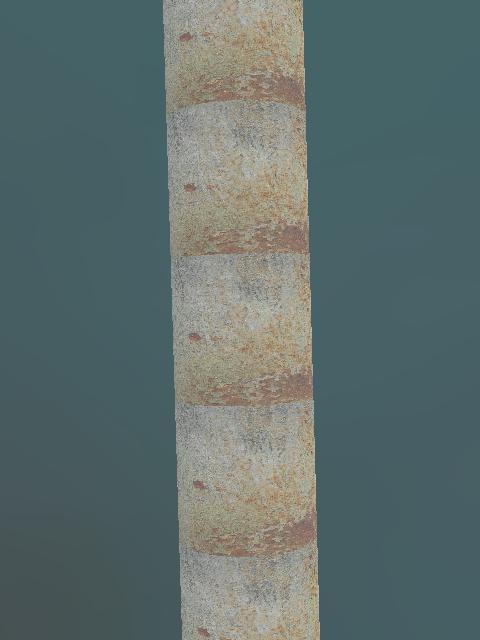
\includegraphics[width=0.5\textwidth,height=0.2\textheight]{/imageProcessing/gradeOptimal.jpg}}&
\subfloat[]{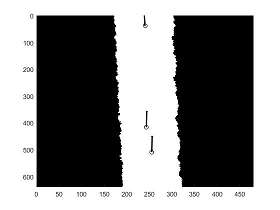
\includegraphics[width=0.5\textwidth,height=0.2\textheight]{/imageProcessing/gradeOptimalFin.jpg}}\\
\subfloat[]{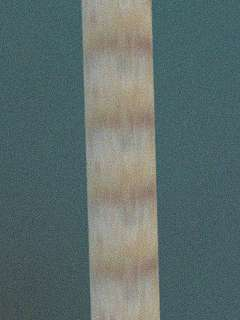
\includegraphics[width=0.5\textwidth,height=0.2\textheight]{/imageProcessing/graeOk.jpg}}&
\subfloat[]{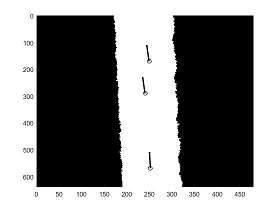
\includegraphics[width=0.5\textwidth,height=0.2\textheight]{/imageProcessing/graeOkFin.jpg}}
\end{tabular}
\caption{Ein gerades Objekt, dass ohne Einschränkungen zu sehen ist wird unter verschiedenen Sichtbedingungen und Bildqualität getestet. }
\end{figure}
\begin{figure}[H]
\begin{tabular}{cc}
\subfloat[]{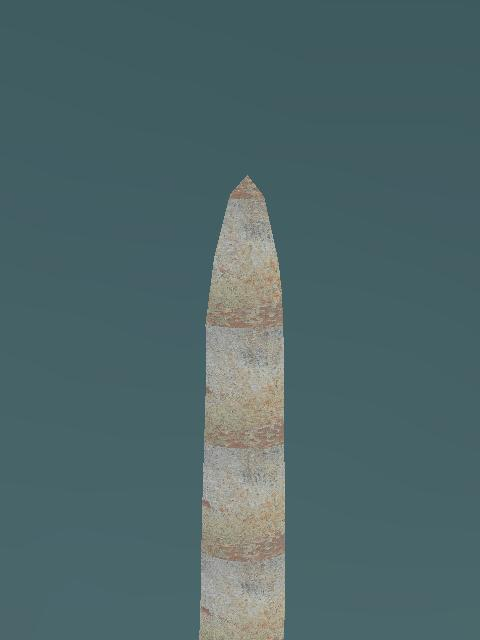
\includegraphics[width=0.5\textwidth,height=0.2\textheight]{/imageProcessing/gradeverborgen.jpg}}&
\subfloat[]{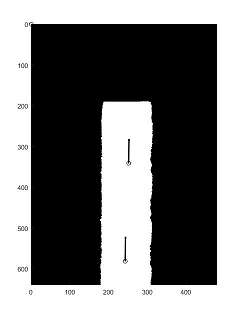
\includegraphics[width=0.5\textwidth,height=0.2\textheight]{/imageProcessing/gradeverborgenfin.jpg}}\\
\subfloat[]{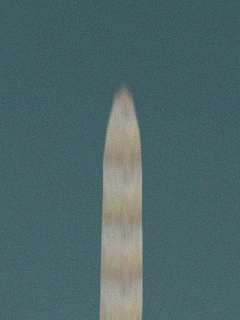
\includegraphics[width=0.5\textwidth,height=0.2\textheight]{/imageProcessing/gradeverborgenok.jpg}}&
\subfloat[]{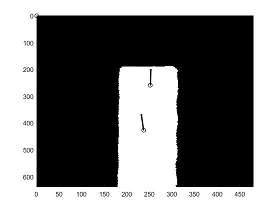
\includegraphics[width=0.5\textwidth,height=0.2\textheight]{/imageProcessing/gradeverborgenokfin.jpg}}
\end{tabular}
\caption{}
\end{figure}
\begin{figure}[H]
\begin{tabular}{cc}
\subfloat[]{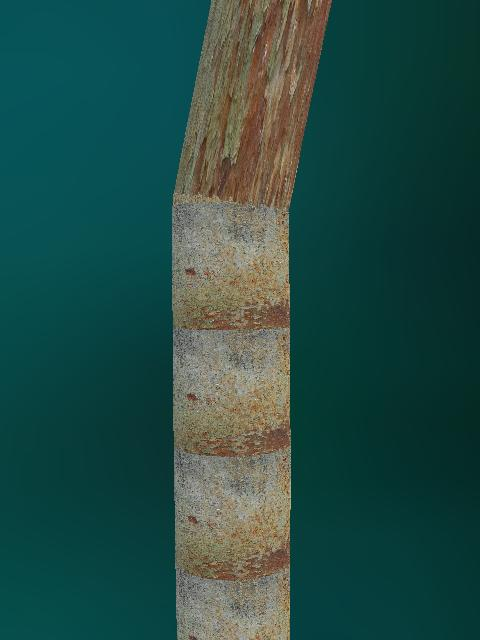
\includegraphics[width=0.5\textwidth,height=0.2\textheight]{/imageProcessing/knickOptimal.jpg}}&
\subfloat[]{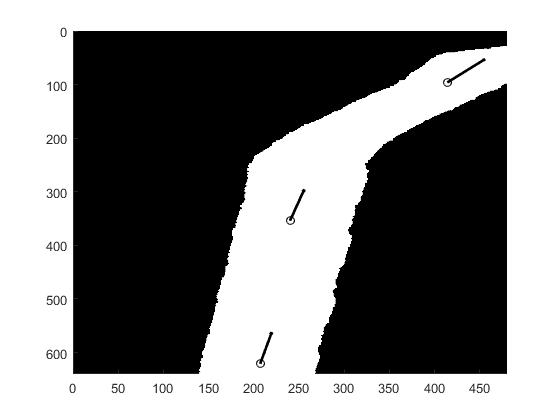
\includegraphics[width=0.5\textwidth,height=0.2\textheight]{/imageProcessing/knickoptimalfin.jpg}}\\
\subfloat[]{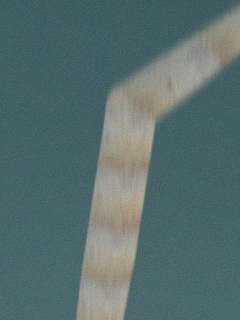
\includegraphics[width=0.5\textwidth,height=0.2\textheight]{/imageProcessing/knickok.jpg}}&
\subfloat[]{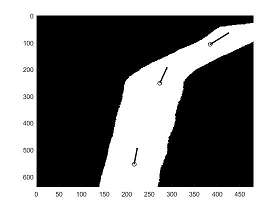
\includegraphics[width=0.5\textwidth,height=0.2\textheight]{/imageProcessing/knickokfin.jpg}}
\end{tabular}
\caption{}
\end{figure}
\begin{figure}[H]
\begin{tabular}{cc}
\subfloat[]{
\includegraphics[width=0.5\textwidth,height=0.2\textheight]{/imageProcessing/nichts.jpg}}&
\subfloat[]{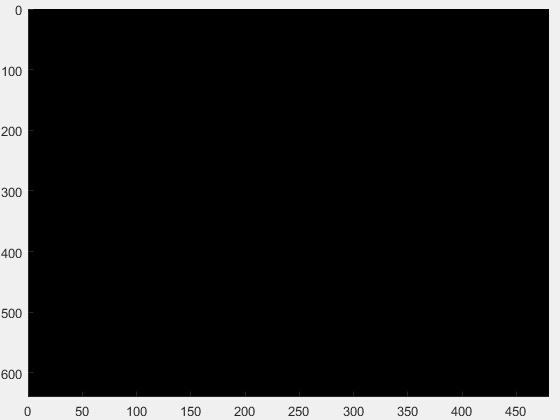
\includegraphics[width=0.5\textwidth,height=0.2\textheight]{/imageProcessing/nichtsoptimalfin.jpg}}\\
\subfloat[]{
\includegraphics[width=0.5\textwidth,height=0.2\textheight]{/imageProcessing/nichtsok.jpg}}&
\subfloat[]{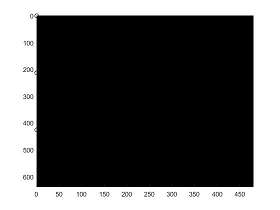
\includegraphics[width=0.5\textwidth,height=0.2\textheight]{/imageProcessing/nichtsokfin.jpg}}
\end{tabular}
\caption{}
\end{figure}

\subsubsection*{Dritte Testreihe}
Um zu testen, ob das Verfahren auch bei echten Bildern funktioniert wurden insgesamt 12 Bilder [Anhang \ref{anhang_objdecttests}] aus einem Testlauf des AUVs \textit{DAGON}\footnote{http://robotik.dfki-bremen.de/de/forschung/robotersysteme/dagon.html} während des Projektes \textit{CUSLAM}\footnote{http://robotik.dfki-bremen.de/de/forschung/projekte/cuslam.html} im Unisee getestet. In einigen Bilder, wie in Abbildung \ref{rp_a} oder \ref{rp_b} ist die Pipeline schwer zu erkennen. Dadurch muss der Schwellwert für das Template entsprechend niedrig gesetzt werden, was in vielen Punkten im Binärbild führt, die nicht zum Objekt gehören. In Bildern, in denen die Pipeline direkt angestrahlt wird und klar heller ist, wie in Abbildung \ref{realData_good} ist das Objekt wieder klar heller als der Hintergrund, der Schwellwert kann höher angesetzt werden um weniger Störpunkte zu erhalten.

\begin{figure}[H]
\begin{tabular}{cc}
\subfloat[]{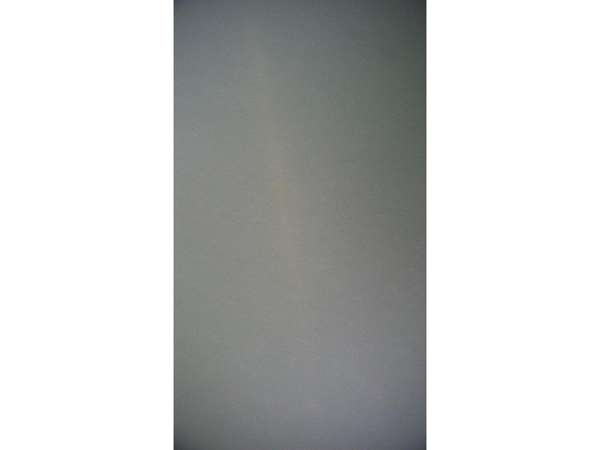
\includegraphics[height=0.2\textheight,width=0.5\textwidth]{imageProcessing/realPipe/001orgImstart.jpg}\label{rp_a}}&
\subfloat[]{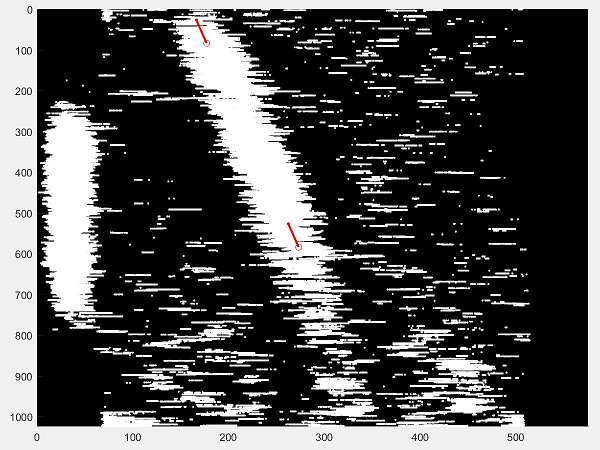
\includegraphics[height=0.2\textheight,width=0.5\textwidth]{imageProcessing/realPipe/001detectedImage.jpg}\label{rp_a}}\\
\subfloat[]{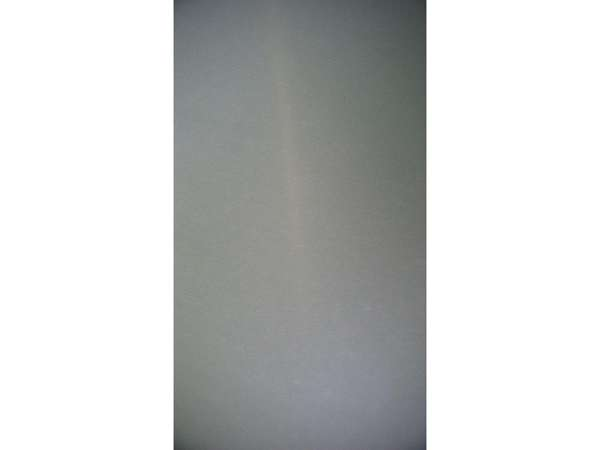
\includegraphics[height=0.2\textheight,width=0.5\textwidth]{imageProcessing/realPipe/002orgImstart.jpg}\label{rp_b}}&
\subfloat[]{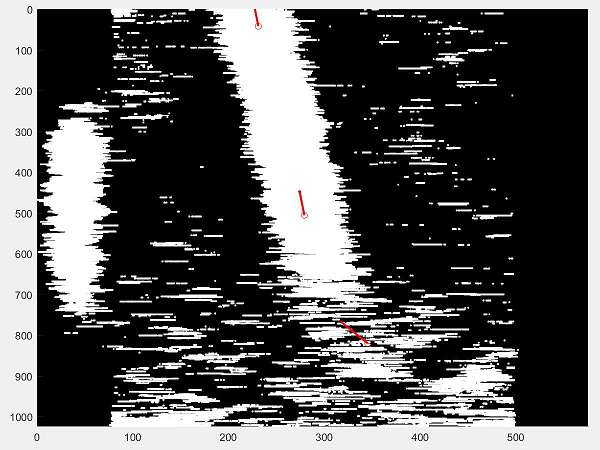
\includegraphics[height=0.2\textheight,width=0.5\textwidth]{imageProcessing/realPipe/002detectedImage.jpg}\label{rp_b}}
\end{tabular}
\caption{Tests der Objekterkennung auf realen Bilder aufgenommen im Unisee vom AUV \textit{DAGON}. Trotz sehr schlechten Sichtbedingungen und vielen Störpunkten im Binärbild wird die Pipeline in den oberen zwei Segmenten gut erkannt. In \textit{d)} ist im unteren Bereich eine Fehldetektion aufgrund der hohen Störpunktdichte in diesem Bereich. Die Randbereiche werden während des Binärisierungsprozess am Bild hinzugefügt, um dass Template auch auf den ersten und letzten Pixeln anwenden zu können. Diese Bereiche werden bei der Detektion nicht betrachtet.}
\label{realData_bad}
\end{figure}

\begin{figure}[H]
\begin{tabular}{cc}
\subfloat[]{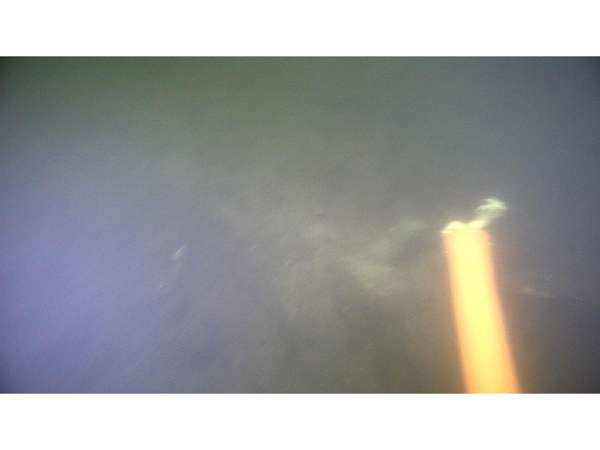
\includegraphics[height=0.2\textheight,width=0.5\textwidth]{imageProcessing/realPipe/008orgImstart.jpg}}&
\subfloat[]{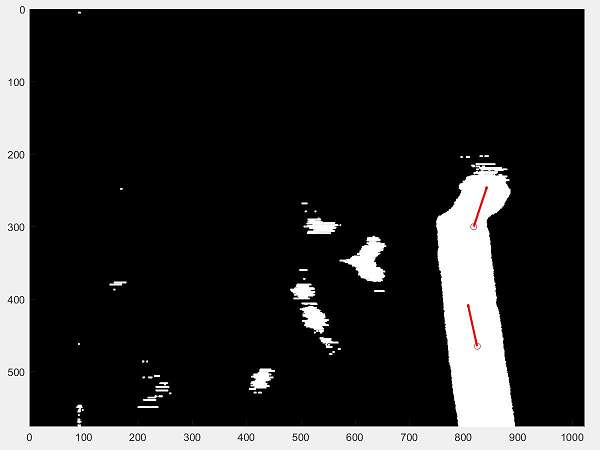
\includegraphics[height=0.2\textheight,width=0.5\textwidth]{imageProcessing/realPipe/008detectedImage.jpg}}\\
\end{tabular}
\caption{Test der Objekterkennung auf einem realen Bild aufgenommen im Unisee vom AUV \textit{DAGON}. Die Pipeline reflektiert sehr stark und hebt sich dadurch deutlich vom Hintergrund ab. Jedoch gibt es eine starke Reflexion des Wassers nah an der Pipeline, was zu einer Fehldetektion im zweiten Segment führt.}
\label{realData_good}
\end{figure}

In den durchgeführten Tests wird deutlich, dass die Objekterkennung unter verschiedensten Sichtbedingungen gute Ergebnisse liefert. Abhängig ist die zuverlässige Detektion vom Templateschwellwert für die Binärisierung des Bildes. Je stärker sich das Objekt vom Hintergrund abhebt, desto höher kann der Schwellwert gewählt werden (vgl. Kapitel \ref{sec_templ}). Bei einem geringen Schwellwert gibt es im Binärbild mehr Störpunkte als bei einem höheren (vgl. Abb. \ref{realData_bad} mit \ref{realData_good}). Für eine zuverlässige Detektion ist 